% Options for packages loaded elsewhere
\PassOptionsToPackage{unicode}{hyperref}
\PassOptionsToPackage{hyphens}{url}
\PassOptionsToPackage{dvipsnames,svgnames,x11names}{xcolor}
\documentclass[
  12pt,
  a4paper,
]{article}
\usepackage{xcolor}
\usepackage[top=2.5cm,bottom=2.5cm,left=3cm,right=2cm]{geometry}
\usepackage{amsmath,amssymb}
\setcounter{secnumdepth}{5}
\usepackage{iftex}
\ifPDFTeX
  \usepackage[T1]{fontenc}
  \usepackage[utf8]{inputenc}
  \usepackage{textcomp} % provide euro and other symbols
\else % if luatex or xetex
  \usepackage{unicode-math} % this also loads fontspec
  \defaultfontfeatures{Scale=MatchLowercase}
  \defaultfontfeatures[\rmfamily]{Ligatures=TeX,Scale=1}
\fi
\usepackage{lmodern}
\ifPDFTeX\else
  % xetex/luatex font selection
    \setmainfont[]{Times New Roman}
    \setmonofont[Scale=0.85]{Liberation Mono}
\fi
% Use upquote if available, for straight quotes in verbatim environments
\IfFileExists{upquote.sty}{\usepackage{upquote}}{}
\IfFileExists{microtype.sty}{% use microtype if available
  \usepackage[]{microtype}
  \UseMicrotypeSet[protrusion]{basicmath} % disable protrusion for tt fonts
}{}
\makeatletter
\@ifundefined{KOMAClassName}{% if non-KOMA class
  \IfFileExists{parskip.sty}{%
    \usepackage{parskip}
  }{% else
    \setlength{\parindent}{0pt}
    \setlength{\parskip}{6pt plus 2pt minus 1pt}}
}{% if KOMA class
  \KOMAoptions{parskip=half}}
\makeatother
\usepackage{color}
\usepackage{fancyvrb}
\newcommand{\VerbBar}{|}
\newcommand{\VERB}{\Verb[commandchars=\\\{\}]}
\DefineVerbatimEnvironment{Highlighting}{Verbatim}{commandchars=\\\{\}}
% Add ',fontsize=\small' for more characters per line
\newenvironment{Shaded}{}{}
\newcommand{\AlertTok}[1]{\textcolor[rgb]{1.00,0.00,0.00}{\textbf{#1}}}
\newcommand{\AnnotationTok}[1]{\textcolor[rgb]{0.38,0.63,0.69}{\textbf{\textit{#1}}}}
\newcommand{\AttributeTok}[1]{\textcolor[rgb]{0.49,0.56,0.16}{#1}}
\newcommand{\BaseNTok}[1]{\textcolor[rgb]{0.25,0.63,0.44}{#1}}
\newcommand{\BuiltInTok}[1]{\textcolor[rgb]{0.00,0.50,0.00}{#1}}
\newcommand{\CharTok}[1]{\textcolor[rgb]{0.25,0.44,0.63}{#1}}
\newcommand{\CommentTok}[1]{\textcolor[rgb]{0.38,0.63,0.69}{\textit{#1}}}
\newcommand{\CommentVarTok}[1]{\textcolor[rgb]{0.38,0.63,0.69}{\textbf{\textit{#1}}}}
\newcommand{\ConstantTok}[1]{\textcolor[rgb]{0.53,0.00,0.00}{#1}}
\newcommand{\ControlFlowTok}[1]{\textcolor[rgb]{0.00,0.44,0.13}{\textbf{#1}}}
\newcommand{\DataTypeTok}[1]{\textcolor[rgb]{0.56,0.13,0.00}{#1}}
\newcommand{\DecValTok}[1]{\textcolor[rgb]{0.25,0.63,0.44}{#1}}
\newcommand{\DocumentationTok}[1]{\textcolor[rgb]{0.73,0.13,0.13}{\textit{#1}}}
\newcommand{\ErrorTok}[1]{\textcolor[rgb]{1.00,0.00,0.00}{\textbf{#1}}}
\newcommand{\ExtensionTok}[1]{#1}
\newcommand{\FloatTok}[1]{\textcolor[rgb]{0.25,0.63,0.44}{#1}}
\newcommand{\FunctionTok}[1]{\textcolor[rgb]{0.02,0.16,0.49}{#1}}
\newcommand{\ImportTok}[1]{\textcolor[rgb]{0.00,0.50,0.00}{\textbf{#1}}}
\newcommand{\InformationTok}[1]{\textcolor[rgb]{0.38,0.63,0.69}{\textbf{\textit{#1}}}}
\newcommand{\KeywordTok}[1]{\textcolor[rgb]{0.00,0.44,0.13}{\textbf{#1}}}
\newcommand{\NormalTok}[1]{#1}
\newcommand{\OperatorTok}[1]{\textcolor[rgb]{0.40,0.40,0.40}{#1}}
\newcommand{\OtherTok}[1]{\textcolor[rgb]{0.00,0.44,0.13}{#1}}
\newcommand{\PreprocessorTok}[1]{\textcolor[rgb]{0.74,0.48,0.00}{#1}}
\newcommand{\RegionMarkerTok}[1]{#1}
\newcommand{\SpecialCharTok}[1]{\textcolor[rgb]{0.25,0.44,0.63}{#1}}
\newcommand{\SpecialStringTok}[1]{\textcolor[rgb]{0.73,0.40,0.53}{#1}}
\newcommand{\StringTok}[1]{\textcolor[rgb]{0.25,0.44,0.63}{#1}}
\newcommand{\VariableTok}[1]{\textcolor[rgb]{0.10,0.09,0.49}{#1}}
\newcommand{\VerbatimStringTok}[1]{\textcolor[rgb]{0.25,0.44,0.63}{#1}}
\newcommand{\WarningTok}[1]{\textcolor[rgb]{0.38,0.63,0.69}{\textbf{\textit{#1}}}}
\usepackage{longtable,booktabs,array}
\usepackage{calc} % for calculating minipage widths
% Correct order of tables after \paragraph or \subparagraph
\usepackage{etoolbox}
\makeatletter
\patchcmd\longtable{\par}{\if@noskipsec\mbox{}\fi\par}{}{}
\makeatother
% Allow footnotes in longtable head/foot
\IfFileExists{footnotehyper.sty}{\usepackage{footnotehyper}}{\usepackage{footnote}}
\makesavenoteenv{longtable}
\usepackage{graphicx}
\makeatletter
\newsavebox\pandoc@box
\newcommand*\pandocbounded[1]{% scales image to fit in text height/width
  \sbox\pandoc@box{#1}%
  \Gscale@div\@tempa{\textheight}{\dimexpr\ht\pandoc@box+\dp\pandoc@box\relax}%
  \Gscale@div\@tempb{\linewidth}{\wd\pandoc@box}%
  \ifdim\@tempb\p@<\@tempa\p@\let\@tempa\@tempb\fi% select the smaller of both
  \ifdim\@tempa\p@<\p@\scalebox{\@tempa}{\usebox\pandoc@box}%
  \else\usebox{\pandoc@box}%
  \fi%
}
% Set default figure placement to htbp
\def\fps@figure{htbp}
\makeatother
\ifLuaTeX
\usepackage[bidi=basic]{babel}
\else
\usepackage[bidi=default]{babel}
\fi
\babelprovide[main,import]{vietnamese}
\ifPDFTeX
\else
\babelfont{rm}[]{Times New Roman}
\fi
% get rid of language-specific shorthands (see #6817):
\let\LanguageShortHands\languageshorthands
\def\languageshorthands#1{}
\setlength{\emergencystretch}{3em} % prevent overfull lines
\providecommand{\tightlist}{%
  \setlength{\itemsep}{0pt}\setlength{\parskip}{0pt}}
\usepackage{fvextra}
\DefineVerbatimEnvironment{Highlighting}{Verbatim}{breaklines,breakanywhere,commandchars=\\\{\}}
\fvset{breaklines,breakanywhere}
\usepackage{float}
\floatplacement{figure}{H}
\usepackage[font=small,labelfont=bf,labelsep=period]{caption}
\usepackage{setspace}
\setstretch{1.2}
\usepackage{fancyhdr}
\pagestyle{fancy}
\fancyhf{}
\fancyhead[L]{\small\nouppercase{\leftmark}}
\fancyhead[R]{\small Báo cáo thực hành Xử lý dữ liệu lớn}
\fancyfoot[C]{\small\thepage}
\renewcommand{\headrulewidth}{0.4pt}
\AtBeginDocument{%
  \renewcommand{\figurename}{Hình}%
  \renewcommand{\tablename}{Bảng}%
  \renewcommand{\contentsname}{Mục lục}%
  \renewcommand{\listfigurename}{Danh mục hình}%
  \renewcommand{\listtablename}{Danh mục bảng}%
  \providecommand{\chaptername}{}\renewcommand{\chaptername}{Chương}%
}
% Symbols missing from Times New Roman: typeset them in math mode instead.
\begingroup
\catcode`⌈=\active \catcode`⌉=\active \catcode`≫=\active \catcode`≪=\active
\protected\gdef⌈{\ensuremath{\lceil}}\protected\gdef⌉{\ensuremath{\rceil}}
\protected\gdef≫{\ensuremath{\gg}}\protected\gdef≪{\ensuremath{\ll}}
\endgroup
\AtBeginDocument{\catcode`⌈=\active \catcode`⌉=\active \catcode`≫=\active \catcode`≪=\active}
\usepackage{bookmark}
\IfFileExists{xurl.sty}{\usepackage{xurl}}{} % add URL line breaks if available
\urlstyle{same}
\hypersetup{
  pdflang={vi},
  colorlinks=true,
  linkcolor={black},
  filecolor={Maroon},
  citecolor={Blue},
  urlcolor={blue},
  pdfcreator={LaTeX via pandoc}}

\author{}
\date{}

\begin{document}

\begin{titlepage}
\centering
{\large\MakeUppercase{Trường Đại học Khoa học Tự nhiên, ĐHQG-HCM}\par}
{\large\bfseries\MakeUppercase{Khoa Toán - Tin học}\par}
\vspace{0.4cm}\rule{0.55\textwidth}{0.6pt}\par
\vspace{1.2cm}
\includegraphics[width=4.5cm]{/data/logo-hcmus.png}\par
\vspace{1.2cm}
{\Large\bfseries BÁO CÁO THỰC HÀNH\par}
\vspace{0.3cm}
{\large Môn học: Xử lý dữ liệu lớn\par}
\vspace{1.5cm}
{\large\bfseries Bài thực hành L01\par}
\vspace{0.4cm}
{\LARGE\bfseries HDFS: tổ chức block, nhân bản và khả năng chịu lỗi
DataNode\par}
\vfill
\begin{tabular}{@{}ll@{}}
Sinh viên thực hiện:  & Nguyễn Thị Huyền Trang \\[2pt]
Mã số sinh viên:      & 23280092 \\[2pt]
Lớp:                  & 23KDL \\
\end{tabular}
\vfill
{\large TP. Hồ Chí Minh, Tháng 10 năm 2026\par}
\end{titlepage}

{
\hypersetup{linkcolor=black}
\setcounter{tocdepth}{3}
\tableofcontents
}
\listoffigures
\listoftables
\section{Mục tiêu và môi trường}\label{sec:l01-intro}

Bài lab dựng một cluster HDFS nhiều node bằng Docker Compose, dùng bộ
lệnh \texttt{hdfs\ dfs}, dùng
\texttt{hdfs\ fsck\ -files\ -blocks\ -locations}\allowbreak{} để xem tệp
được chia thành block và replica, thay đổi block size và hệ số nhân bản,
dừng một DataNode để quan sát under-replication và tái nhân bản, cuối
cùng thử safe mode và đọc fsimage.

Cluster chạy trên một máy (Bảng~\ref{tbl:l01-env}).
\texttt{recheck-interval}\allowbreak{} được rút xuống 30 s để thấy sự cố
DataNode trong khoảng 90 s thay vì hơn 10 phút. Mọi lệnh chạy trong
container \texttt{namenode} (đóng vai trò edge node), trừ
\texttt{docker\ compose} chạy trên host.

\begin{longtable}[]{@{}
  >{\raggedright\arraybackslash}p{(\linewidth - 2\tabcolsep) * \real{0.5000}}
  >{\raggedright\arraybackslash}p{(\linewidth - 2\tabcolsep) * \real{0.5000}}@{}}
\caption{\label{tbl:l01-env}Phần cứng, phần mềm và cấu hình HDFS dùng
trong thực nghiệm.}\tabularnewline
\toprule\noalign{}
\begin{minipage}[b]{\linewidth}\raggedright
Thành phần
\end{minipage} & \begin{minipage}[b]{\linewidth}\raggedright
Giá trị
\end{minipage} \\
\midrule\noalign{}
\endfirsthead
\toprule\noalign{}
\begin{minipage}[b]{\linewidth}\raggedright
Thành phần
\end{minipage} & \begin{minipage}[b]{\linewidth}\raggedright
Giá trị
\end{minipage} \\
\midrule\noalign{}
\endhead
\bottomrule\noalign{}
\endlastfoot
Máy chủ & WSL2, x86\_64, 12 CPU, bộ nhớ Docker 31.9 GB \\
Phần mềm & Hadoop 3.4.3 (image
\texttt{de-labs/}\allowbreak{}\texttt{hadoop:}\allowbreak{}\texttt{3.}\allowbreak{}\texttt{4.}\allowbreak{}\texttt{3}\allowbreak{}),
Docker Compose \\
Dịch vụ & 1 NameNode, 3 DataNode, ResourceManager, NodeManager,
JobHistory \\
Topology & 1 rack (\texttt{/default-rack}) \\
\texttt{dfs.replication} & 3 \\
\texttt{dfs.blocksize} & 134,217,728 byte (128 MB, mặc định) \\
\texttt{dfs.}\allowbreak{}\texttt{heartbeat.}\allowbreak{}\texttt{interval}\allowbreak{}
& 3 s \\
\texttt{dfs.}\allowbreak{}\texttt{namenode.}\allowbreak{}\texttt{heartbeat.}\allowbreak{}\texttt{recheck-interval}\allowbreak{}
& 30,000 ms (mặc định 300,000 ms) \\
\texttt{dfs.}\allowbreak{}\texttt{namenode.}\allowbreak{}\texttt{stale.}\allowbreak{}\texttt{datanode.}\allowbreak{}\texttt{interval}\allowbreak{}
& 15,000 ms (mặc định 30,000 ms) \\
\texttt{dfs.}\allowbreak{}\texttt{namenode.}\allowbreak{}\texttt{redundancy.}\allowbreak{}\texttt{interval.}\allowbreak{}\texttt{seconds}\allowbreak{}
& 3 s \\
\texttt{dfs.}\allowbreak{}\texttt{namenode.}\allowbreak{}\texttt{safemode.}\allowbreak{}\texttt{extension}\allowbreak{}
& 5,000 ms (mặc định 30,000 ms) \\
\texttt{dfs.}\allowbreak{}\texttt{permissions.}\allowbreak{}\texttt{enabled}\allowbreak{}
& false (chỉ dùng cho môi trường học tập) \\
\end{longtable}

Dữ liệu là hai tệp NYC Taxi đọc từ thư mục \texttt{/datasets} bind mount
vào container:
\texttt{taxi\_}\allowbreak{}\texttt{zone\_}\allowbreak{}\texttt{lookup.}\allowbreak{}\texttt{csv}\allowbreak{}
(12,331 byte) và
\texttt{yellow\_}\allowbreak{}\texttt{tripdata\_}\allowbreak{}\texttt{2024-01.}\allowbreak{}\texttt{parquet}\allowbreak{}
(49,961,641 byte, \texttt{hdfs\ dfs\ -du\ -h} hiển thị 47.6 M).

\section{Thực hiện và kết quả}\label{sec:l01-results}

\subsection{Khởi động cluster}\label{sec:l01-cluster}

Sau khi khởi động, \texttt{hdfs\ dfsadmin\ -report}\allowbreak{} ghi
nhận \texttt{Live\ datanodes\ (3)}\allowbreak{}, safe mode OFF. Vì
\texttt{fsck} in vị trí replica theo IP, chúng tôi ghi lại ánh xạ IP
sang hostname ngay lúc này (Bảng~\ref{tbl:l01-ip}). Block Pool ID
\texttt{BP-361839436-172.}\allowbreak{}\texttt{29.}\allowbreak{}\texttt{0.}\allowbreak{}\texttt{7-1793355266756}\allowbreak{}
cho biết NameNode ở 172.29.0.7.

\begin{longtable}[]{@{}ll@{}}
\caption{\label{tbl:l01-ip}Ánh xạ địa chỉ IP sang hostname của các
DataNode.}\tabularnewline
\toprule\noalign{}
Địa chỉ IP & Hostname \\
\midrule\noalign{}
\endfirsthead
\toprule\noalign{}
Địa chỉ IP & Hostname \\
\midrule\noalign{}
\endhead
\bottomrule\noalign{}
\endlastfoot
172.29.0.5 & datanode1 \\
172.29.0.2 & datanode2 \\
172.29.0.3 & datanode3 \\
\end{longtable}

Trên giao diện web cổng 9870, trang Overview báo NameNode
\texttt{active}, phiên bản 3.4.3, safe mode tắt, 3 node sống, 0 node
chết, 0 block under-replicated (Hình~\ref{fig:l01-ui-overview}). Trang
Datanodes liệt kê cả ba node ở trạng thái In service
(Hình~\ref{fig:l01-ui-datanodes}).

\begin{figure}
\centering
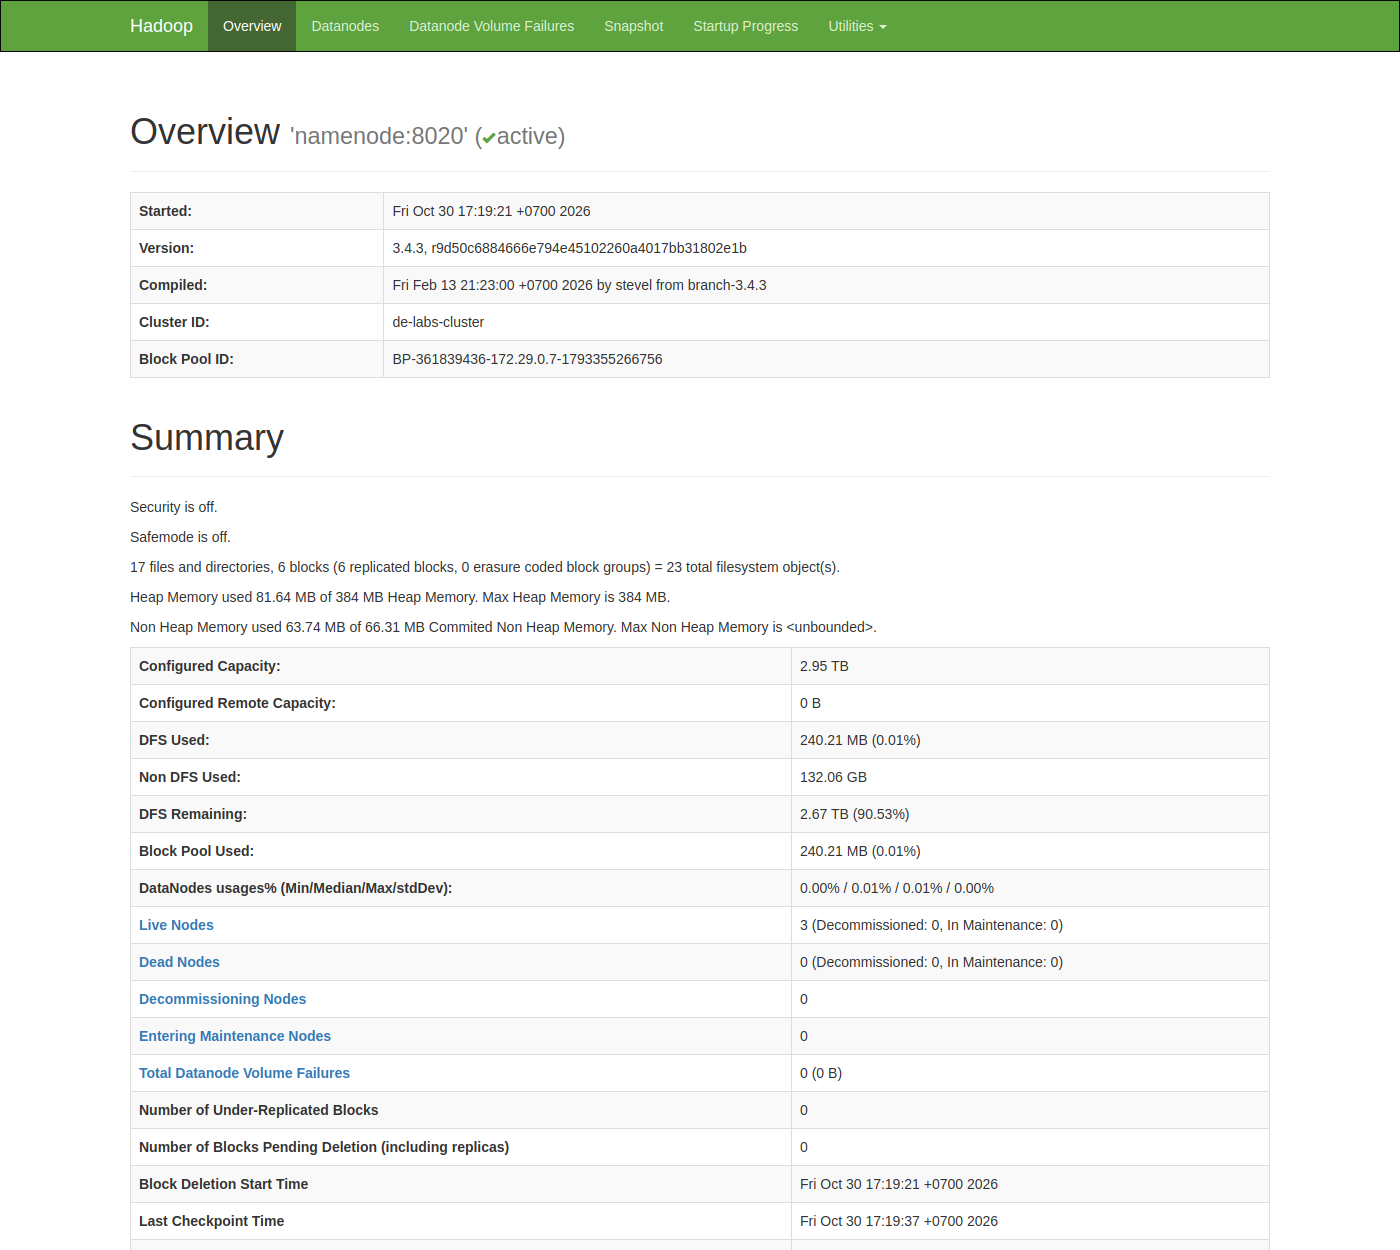
\includegraphics[width=1\linewidth,height=\textheight,keepaspectratio]{img/11_ui_namenode_overview_healthy.png}
\caption{Trang Overview của NameNode khi cluster khỏe mạnh: 3 Live
Nodes, 0 Dead Nodes, 0 block
under-replicated.}\label{fig:l01-ui-overview}
\end{figure}

\begin{figure}
\centering
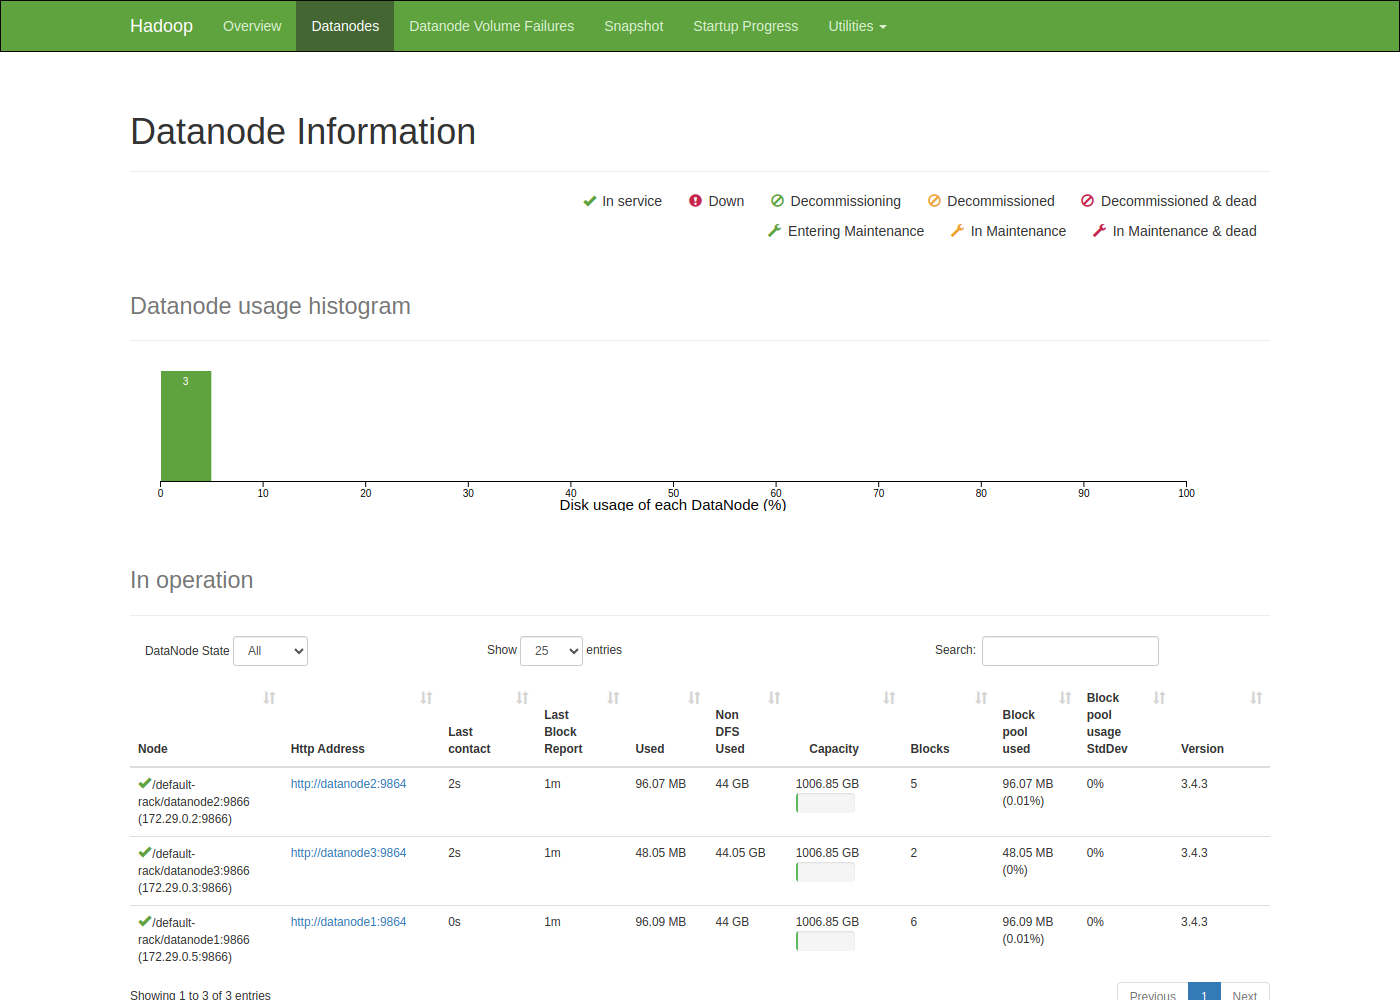
\includegraphics[width=1\linewidth,height=\textheight,keepaspectratio]{img/12_ui_datanodes_healthy.png}
\caption{Trang Datanodes của NameNode khi cả ba DataNode đều ở trạng
thái In service.}\label{fig:l01-ui-datanodes}
\end{figure}

\subsection{\texorpdfstring{Bộ lệnh
\texttt{hdfs\ dfs}}{Bộ lệnh hdfs dfs}}\label{sec:l01-shell}

Các lệnh \texttt{hdfs\ dfs} đều chạy được (Hình~\ref{fig:l01-shell}).
\texttt{taxi\_}\allowbreak{}\texttt{zone\_}\allowbreak{}\texttt{lookup.}\allowbreak{}\texttt{csv}\allowbreak{}
có hệ số 3 (cột thứ hai của \texttt{ls}), \texttt{cat} kết hợp
\texttt{grep\ -c} đếm được 70 dòng Manhattan, bản tải về
\texttt{/}\allowbreak{}\texttt{tmp/}\allowbreak{}\texttt{zones\_}\allowbreak{}\texttt{copy.}\allowbreak{}\texttt{csv}\allowbreak{}
đúng 12,331 byte. \texttt{du\ -h} in 12.0 K dung lượng logic và 36.1 K
dung lượng thô, gấp ba do nhân bản. Lệnh \texttt{hdfs\ dfs\ -stat} (Phụ
lục) trả về
\texttt{blocksize=}\allowbreak{}\texttt{134217728\ repl=}\allowbreak{}\texttt{3\ size=}\allowbreak{}\texttt{12331}\allowbreak{}:
tệp 12 KB vẫn được gán block size 128 MB.

\begin{figure}
\centering
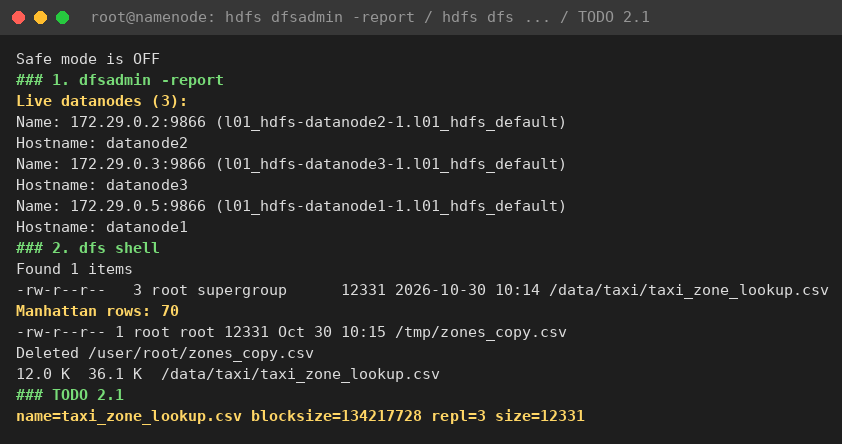
\includegraphics[width=0.85\linewidth,height=\textheight,keepaspectratio]{img/01_cluster_and_dfs_shell.png}
\caption{Đầu ra \texttt{dfsadmin\ -report}\allowbreak{} (3 DataNode
sống, ánh xạ IP sang hostname), chuỗi lệnh \texttt{hdfs\ dfs} và kết quả
\texttt{hdfs\ dfs\ -stat}.}\label{fig:l01-shell}
\end{figure}

\subsection{Block size mặc định và block 16 MB}\label{sec:l01-blocksize}

Tệp Parquet được tải lên hai lần: block mặc định vào
\texttt{/}\allowbreak{}\texttt{data/}\allowbreak{}\texttt{taxi/}\allowbreak{}\texttt{default\_}\allowbreak{}\texttt{blocks}\allowbreak{}
và
\texttt{-D\ dfs.}\allowbreak{}\texttt{blocksize=}\allowbreak{}\texttt{16m}\allowbreak{}
vào
\texttt{/}\allowbreak{}\texttt{data/}\allowbreak{}\texttt{taxi/}\allowbreak{}\texttt{small\_}\allowbreak{}\texttt{blocks}\allowbreak{}.
\texttt{hdfs\ dfs\ -stat} cho bản thứ nhất
\texttt{blocksize=}\allowbreak{}\texttt{134217728}\allowbreak{}, bản thứ
hai \texttt{blocksize=}\allowbreak{}\texttt{16777216}\allowbreak{}, cả
hai \texttt{repl=3}. Block size chỉ là giới hạn trên, block cuối chỉ lớn
bằng phần dữ liệu còn lại {[}3{]}. Kết quả \texttt{fsck} ở
Bảng~\ref{tbl:l01-blocks} và Hình~\ref{fig:l01-blocks}; trang Browse
Directory cũng hiển thị \texttt{default\_blocks}, \texttt{small\_blocks}
và
\texttt{taxi\_}\allowbreak{}\texttt{zone\_}\allowbreak{}\texttt{lookup.}\allowbreak{}\texttt{csv}\allowbreak{}
trong \texttt{/data/taxi} với Replication 3, Block Size 128 MB
(Hình~\ref{fig:l01-ui-browse}).

\begin{longtable}[]{@{}
  >{\raggedright\arraybackslash}p{(\linewidth - 6\tabcolsep) * \real{0.2500}}
  >{\raggedright\arraybackslash}p{(\linewidth - 6\tabcolsep) * \real{0.2500}}
  >{\raggedright\arraybackslash}p{(\linewidth - 6\tabcolsep) * \real{0.2500}}
  >{\raggedright\arraybackslash}p{(\linewidth - 6\tabcolsep) * \real{0.2500}}@{}}
\caption{\label{tbl:l01-blocks}Số block của cùng một tệp khi dùng block
128 MB và 16 MB.}\tabularnewline
\toprule\noalign{}
\begin{minipage}[b]{\linewidth}\raggedright
Cách tải lên
\end{minipage} & \begin{minipage}[b]{\linewidth}\raggedright
Block size (byte)
\end{minipage} & \begin{minipage}[b]{\linewidth}\raggedright
Số block
\end{minipage} & \begin{minipage}[b]{\linewidth}\raggedright
Kích thước từng block (byte)
\end{minipage} \\
\midrule\noalign{}
\endfirsthead
\toprule\noalign{}
\begin{minipage}[b]{\linewidth}\raggedright
Cách tải lên
\end{minipage} & \begin{minipage}[b]{\linewidth}\raggedright
Block size (byte)
\end{minipage} & \begin{minipage}[b]{\linewidth}\raggedright
Số block
\end{minipage} & \begin{minipage}[b]{\linewidth}\raggedright
Kích thước từng block (byte)
\end{minipage} \\
\midrule\noalign{}
\endhead
\bottomrule\noalign{}
\endlastfoot
Mặc định & 134,217,728 & 1 & 49,961,641 \\
\texttt{-D\ dfs.}\allowbreak{}\texttt{blocksize=}\allowbreak{}\texttt{16m}\allowbreak{}
& 16,777,216 & 3 & 16,777,216 + 16,777,216 + 16,407,209 \\
\end{longtable}

\begin{figure}
\centering
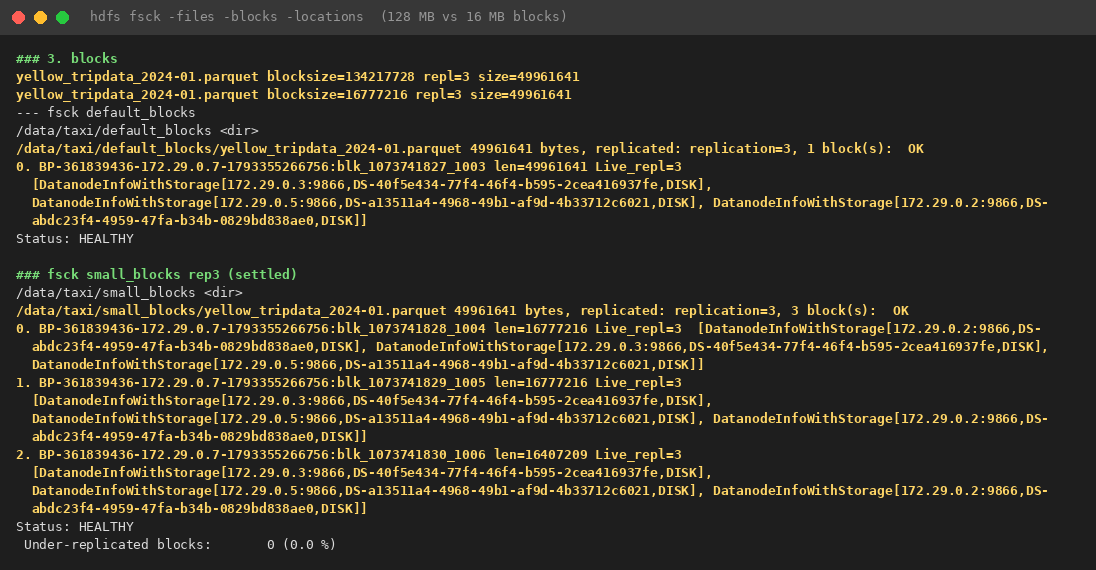
\includegraphics[width=0.85\linewidth,height=\textheight,keepaspectratio]{img/02_blocks_128m_vs_16m.png}
\caption{Kết quả \texttt{fsck\ -files\ -blocks\ -locations}\allowbreak{}
của tệp Parquet với block mặc định (1 block) và block 16 MB (3
block).}\label{fig:l01-blocks}
\end{figure}

\begin{figure}
\centering
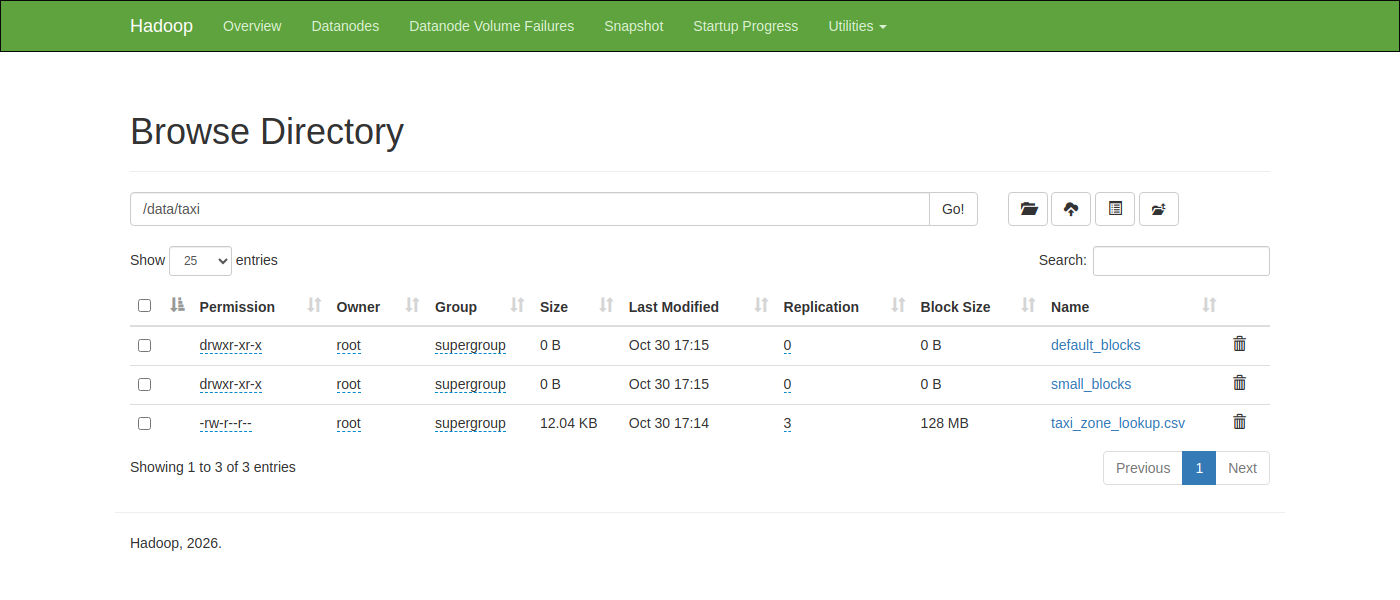
\includegraphics[width=1\linewidth,height=\textheight,keepaspectratio]{img/13_ui_browse_data_taxi.png}
\caption{Trang Browse Directory hiển thị thư mục \texttt{/data/taxi} với
hệ số nhân bản và block size của từng mục.}\label{fig:l01-ui-browse}
\end{figure}

Ở lần \texttt{fsck} đầu tiên trên \texttt{small\_blocks} (10:15:21, ngay
sau khi ghi), hai block \texttt{blk\_1073741829} và
\texttt{blk\_1073741830} chỉ có \texttt{Live\_repl=2}, kèm
\texttt{Under-replicated\ blocks:}\allowbreak{}\texttt{\ 2\ (66.}\allowbreak{}\texttt{666664\ \%)}\allowbreak{}
và
\texttt{Missing\ replicas:}\allowbreak{}\texttt{\ 2\ (22.}\allowbreak{}\texttt{222221\ \%)}\allowbreak{},
dù trạng thái vẫn \texttt{HEALTHY}. Lúc đầu chúng tôi nghĩ việc ghi bị
lỗi, nhưng lần \texttt{fsck} tiếp theo (đầu tệp \texttt{02\_setrep.txt})
đã cho cả ba block \texttt{Live\_repl=3} và
\texttt{Under-replicated\ blocks:}\allowbreak{}\texttt{\ 0}\allowbreak{}.
NameNode chỉ cập nhật vị trí replica khi DataNode báo về, nên sau khi
ghi có một khoảng trễ ngắn.

Trên datanode1, mỗi block là một tệp
\texttt{blk\_\textless{}id\textgreater{}} kèm tệp
\texttt{blk\_}\allowbreak{}\texttt{\textless{}id\textgreater{}\_}\allowbreak{}\texttt{\textless{}genstamp\textgreater{}.}\allowbreak{}\texttt{meta}\allowbreak{}
chứa checksum (Hình~\ref{fig:l01-physical},
Bảng~\ref{tbl:l01-physical}). Block cuối chỉ có 16,407,209 byte, không
bị đệm lên 16 MB. Tệp \texttt{.meta} 131,079 byte của block 16,777,216
byte khớp với 4 byte CRC cho mỗi 512 byte dữ liệu
(\(16{,}777{,}216 / 512 \times 4 = 131{,}072\)) cộng 7 byte header, tức
chi phí checksum khoảng 0.78 \%.

\begin{longtable}[]{@{}
  >{\raggedright\arraybackslash}p{(\linewidth - 6\tabcolsep) * \real{0.2500}}
  >{\raggedright\arraybackslash}p{(\linewidth - 6\tabcolsep) * \real{0.2500}}
  >{\raggedright\arraybackslash}p{(\linewidth - 6\tabcolsep) * \real{0.2500}}
  >{\raggedright\arraybackslash}p{(\linewidth - 6\tabcolsep) * \real{0.2500}}@{}}
\caption{\label{tbl:l01-physical}Các tệp block vật lý trên datanode1 và
tệp checksum đi kèm.}\tabularnewline
\toprule\noalign{}
\begin{minipage}[b]{\linewidth}\raggedright
Tệp block
\end{minipage} & \begin{minipage}[b]{\linewidth}\raggedright
Dữ liệu (byte)
\end{minipage} & \begin{minipage}[b]{\linewidth}\raggedright
\texttt{.meta} (byte)
\end{minipage} & \begin{minipage}[b]{\linewidth}\raggedright
Thuộc tệp
\end{minipage} \\
\midrule\noalign{}
\endfirsthead
\toprule\noalign{}
\begin{minipage}[b]{\linewidth}\raggedright
Tệp block
\end{minipage} & \begin{minipage}[b]{\linewidth}\raggedright
Dữ liệu (byte)
\end{minipage} & \begin{minipage}[b]{\linewidth}\raggedright
\texttt{.meta} (byte)
\end{minipage} & \begin{minipage}[b]{\linewidth}\raggedright
Thuộc tệp
\end{minipage} \\
\midrule\noalign{}
\endhead
\bottomrule\noalign{}
\endlastfoot
\texttt{blk\_1073741825} & 12,331 & 107 &
\texttt{taxi\_}\allowbreak{}\texttt{zone\_}\allowbreak{}\texttt{lookup.}\allowbreak{}\texttt{csv}\allowbreak{} \\
\texttt{blk\_1073741827} & 49,961,641 & 390,335 &
\texttt{default\_}\allowbreak{}\texttt{blocks/}\allowbreak{}\texttt{.}\allowbreak{}\texttt{.}\allowbreak{}\texttt{.}\allowbreak{}\texttt{parquet}\allowbreak{} \\
\texttt{blk\_1073741828} & 16,777,216 & 131,079 &
\texttt{small\_}\allowbreak{}\texttt{blocks/}\allowbreak{}\texttt{.}\allowbreak{}\texttt{.}\allowbreak{}\texttt{.}\allowbreak{}\texttt{parquet}\allowbreak{},
block 0 \\
\texttt{blk\_1073741829} & 16,777,216 & 131,079 &
\texttt{small\_}\allowbreak{}\texttt{blocks/}\allowbreak{}\texttt{.}\allowbreak{}\texttt{.}\allowbreak{}\texttt{.}\allowbreak{}\texttt{parquet}\allowbreak{},
block 1 \\
\texttt{blk\_1073741830} & 16,407,209 & 128,191 &
\texttt{small\_}\allowbreak{}\texttt{blocks/}\allowbreak{}\texttt{.}\allowbreak{}\texttt{.}\allowbreak{}\texttt{.}\allowbreak{}\texttt{parquet}\allowbreak{},
block 2 \\
\end{longtable}

\begin{figure}
\centering
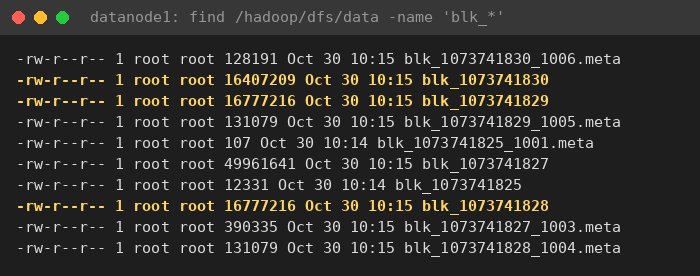
\includegraphics[width=0.85\linewidth,height=\textheight,keepaspectratio]{img/03_physical_block_files_datanode1.png}
\caption{Tệp block vật lý \texttt{blk\_\textless{}id\textgreater{}} và
\texttt{blk\_}\allowbreak{}\texttt{\textless{}id\textgreater{}\_}\allowbreak{}\texttt{\textless{}genstamp\textgreater{}.}\allowbreak{}\texttt{meta}\allowbreak{}
trong thư mục dữ liệu của datanode1.}\label{fig:l01-physical}
\end{figure}

\subsection{Thay đổi hệ số nhân bản}\label{sec:l01-setrep}

\texttt{hdfs\ dfs\ -setrep\ -w\ 2}\allowbreak{} trên tệp
\texttt{small\_blocks} in cảnh báo rằng việc giảm hệ số có thể phải chờ
lâu, nhưng thực tế kết thúc gần như ngay (\texttt{.\ done}). Sau đó
\texttt{ls} hiển thị hệ số 2 và \texttt{fsck} cho \texttt{Live\_repl=2}
ở cả ba block. Dung lượng thô của \texttt{small\_blocks} giảm đúng một
phần ba so với bản \texttt{default\_blocks} còn hệ số 3
(Bảng~\ref{tbl:l01-du}).

\begin{longtable}[]{@{}llll@{}}
\caption{\label{tbl:l01-du}Dung lượng logic và dung lượng thô theo
\texttt{hdfs\ dfs\ -du\ -h} sau khi \texttt{setrep\ 2}.}\tabularnewline
\toprule\noalign{}
Đường dẫn & Hệ số & Dung lượng logic & Dung lượng thô \\
\midrule\noalign{}
\endfirsthead
\toprule\noalign{}
Đường dẫn & Hệ số & Dung lượng logic & Dung lượng thô \\
\midrule\noalign{}
\endhead
\bottomrule\noalign{}
\endlastfoot
\texttt{/}\allowbreak{}\texttt{data/}\allowbreak{}\texttt{taxi/}\allowbreak{}\texttt{default\_}\allowbreak{}\texttt{blocks}\allowbreak{}
& 3 & 47.6 M & 142.9 M \\
\texttt{/}\allowbreak{}\texttt{data/}\allowbreak{}\texttt{taxi/}\allowbreak{}\texttt{small\_}\allowbreak{}\texttt{blocks}\allowbreak{}
& 2 & 47.6 M & 95.3 M \\
\texttt{/}\allowbreak{}\texttt{data/}\allowbreak{}\texttt{taxi/}\allowbreak{}\texttt{taxi\_}\allowbreak{}\texttt{zone\_}\allowbreak{}\texttt{lookup.}\allowbreak{}\texttt{csv}\allowbreak{}
& 3 & 12.0 K & 36.1 K \\
\end{longtable}

Hệ số nhân bản là tham số phía client, nên để ghi tệp với một replica mà
không cần \texttt{setrep} chỉ cần ghi đè
\texttt{-D\ dfs.}\allowbreak{}\texttt{replication=}\allowbreak{}\texttt{1}\allowbreak{}
ngay trong lệnh \texttt{put} (Phụ lục). Kết quả là
\texttt{one\_}\allowbreak{}\texttt{replica.}\allowbreak{}\texttt{csv\ repl=}\allowbreak{}\texttt{1}\allowbreak{},
block duy nhất \texttt{blk\_1073741831} (12,331 byte,
\texttt{Live\_repl=1}) nằm trên 172.29.0.5, tức datanode1
(Hình~\ref{fig:l01-setrep}).

\begin{figure}
\centering
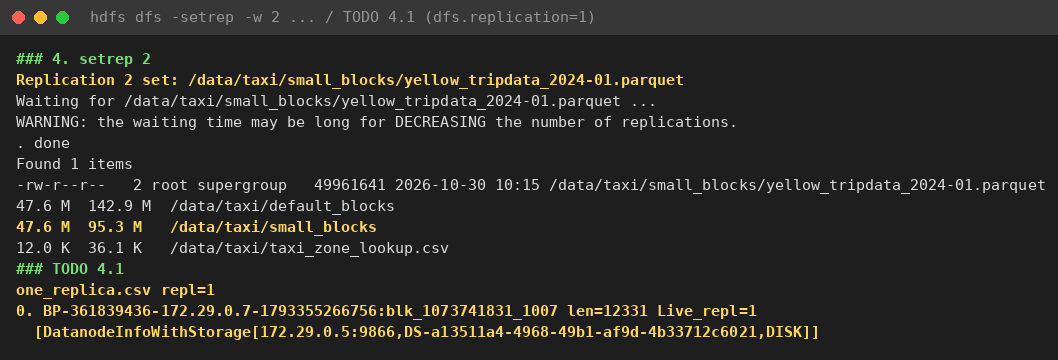
\includegraphics[width=0.85\linewidth,height=\textheight,keepaspectratio]{img/04_setrep2_and_todo4.1.png}
\caption{Kết quả \texttt{setrep\ -w\ 2}, \texttt{du\ -h} sau khi giảm hệ
số và tệp được ghi với hệ số nhân bản 1.}\label{fig:l01-setrep}
\end{figure}

\subsection{Dừng một DataNode và tái nhân bản}\label{sec:l01-failure}

Ngay trước khi dừng node (10:15:58), cả ba block của
\texttt{small\_blocks} đều có replica trên datanode1 và datanode3, không
block nào nằm trên datanode2 (Hình~\ref{fig:l01-before}, cột ``Trước sự
cố'' của Bảng~\ref{tbl:l01-locations}). Vì vậy chúng tôi chọn dừng
datanode3: node này giữ replica của mọi block thuộc tệp hệ số 2.

\begin{figure}
\centering
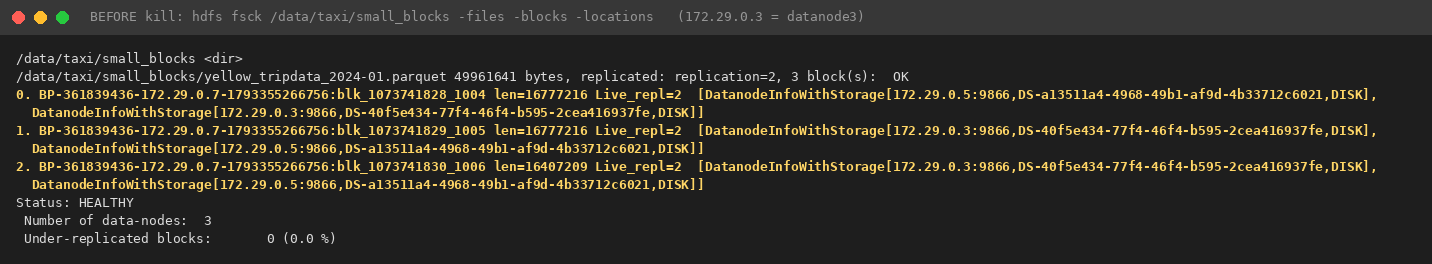
\includegraphics[width=0.85\linewidth,height=\textheight,keepaspectratio]{img/05_fsck_small_blocks_BEFORE_kill.png}
\caption{\texttt{fsck} của tệp block 16 MB trước khi dừng datanode3: mỗi
block có 2 replica trên datanode1 và datanode3.}\label{fig:l01-before}
\end{figure}

Datanode3 bị dừng bằng \texttt{docker\ compose\ stop}\allowbreak{} lúc
10:16:06 UTC, sau đó \texttt{hdfs\ dfsadmin\ -report}\allowbreak{} được
thăm dò trong vòng lặp \texttt{sleep\ 5} (chu kỳ thực tế khoảng 8 s).
DataNode gửi heartbeat mỗi 3 s; node im lặng bị coi là dead sau

\[T_{dead} = 2 \times \text{recheck-interval} + 10 \times \text{heartbeat-interval}\]

{[}5{]}. Với cấu hình lab, \(T_{dead} = 2 \times 30 + 10 \times 3 = 90\)
s. Diễn biến đo được ở Bảng~\ref{tbl:l01-timeline} và
Hình~\ref{fig:l01-timeline}.

\begin{longtable}[]{@{}
  >{\raggedright\arraybackslash}p{(\linewidth - 2\tabcolsep) * \real{0.5000}}
  >{\raggedright\arraybackslash}p{(\linewidth - 2\tabcolsep) * \real{0.5000}}@{}}
\caption{\label{tbl:l01-timeline}Diễn biến sau khi dừng datanode3 theo
\texttt{dfsadmin\ -report}\allowbreak{} và log NameNode.}\tabularnewline
\toprule\noalign{}
\begin{minipage}[b]{\linewidth}\raggedright
Thời điểm
\end{minipage} & \begin{minipage}[b]{\linewidth}\raggedright
Sự kiện
\end{minipage} \\
\midrule\noalign{}
\endfirsthead
\toprule\noalign{}
\begin{minipage}[b]{\linewidth}\raggedright
Thời điểm
\end{minipage} & \begin{minipage}[b]{\linewidth}\raggedright
Sự kiện
\end{minipage} \\
\midrule\noalign{}
\endhead
\bottomrule\noalign{}
\endlastfoot
t+0 s (10:16:06) &
\texttt{docker\ compose\ stop\ datanode3}\allowbreak{} \\
t+1 s đến t+82 s & \texttt{Live\ datanodes\ (3)}\allowbreak{},
\texttt{Under\ replicated\ blocks:}\allowbreak{}\texttt{\ 0}\allowbreak{}
(11 lần thăm dò) \\
t+90 s & \texttt{Live\ datanodes\ (2)}\allowbreak{},
\texttt{Dead\ datanodes\ (1)}\allowbreak{}: node bị tuyên bố chết \\
t+94 s (10:17:40,079) & Log NameNode:
\texttt{removeDeadDatanode:}\allowbreak{}\texttt{\ lost\ heartbeat\ from\ 172.}\allowbreak{}\texttt{29.}\allowbreak{}\texttt{0.}\allowbreak{}\texttt{3:}\allowbreak{}\texttt{9866}\allowbreak{} \\
t+98 s đến t+137 s &
\texttt{Under\ replicated\ blocks:}\allowbreak{}\texttt{\ 2}\allowbreak{}
ổn định qua 6 lần thăm dò \\
\end{longtable}

\begin{figure}
\centering
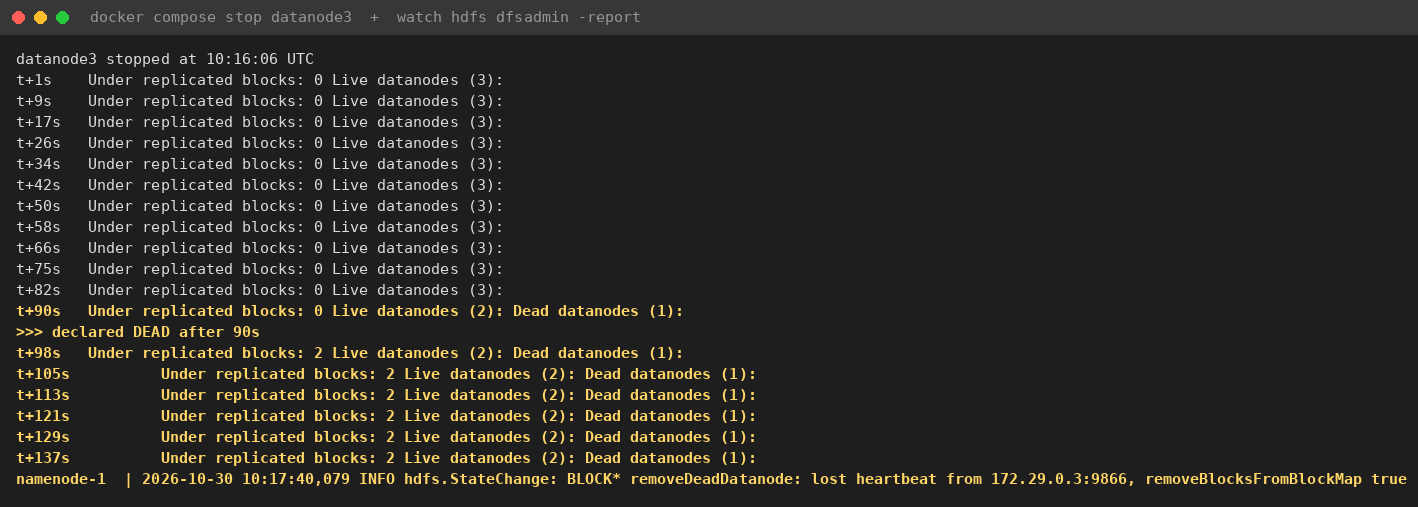
\includegraphics[width=0.85\linewidth,height=\textheight,keepaspectratio]{img/06_kill_datanode3_timeline.png}
\caption{Dòng thời gian thăm dò \texttt{dfsadmin\ -report}\allowbreak{}
sau khi dừng datanode3 và dòng log
\texttt{removeDeadDatanode}\allowbreak{} của
NameNode.}\label{fig:l01-timeline}
\end{figure}

Node bị tuyên bố chết đúng sau \textbf{90 s}, khớp công thức. Replica bị
gỡ khỏi block map muộn hơn 4 s vì bộ giám sát heartbeat chỉ chạy theo
chu kỳ recheck-interval, và phải sau mốc này chỉ số under-replicated mới
tăng. Có một điểm lúc đầu chúng tôi thấy lạ: ba block của tệp hệ số 2
cũng mất một replica, nhưng không lần thăm dò nào ghi nhận quá 2 block
under-replicated. Cách giải thích hợp lý là ba block đó đã được tái nhân
bản trong khoảng t+94 s đến t+98 s, nhanh hơn chu kỳ thăm dò. Giá trị 2
còn lại là hai block của các tệp hệ số 3 (Bảng~\ref{tbl:l01-underrep}).

Trên giao diện web, trang Overview hiện một Dead Node
(Hình~\ref{fig:l01-ui-dead-overview}) và trang Datanodes đánh dấu
datanode3 màu đỏ kèm thời điểm liên lạc cuối
(Hình~\ref{fig:l01-ui-dead-datanodes}). Lần đo chính chúng tôi không kịp
chụp giao diện, nên hai ảnh này được chụp ở một lần dừng datanode3 khác;
mốc ``Last contact'' 17:21:04 +0700 (10:21:04 UTC) muộn hơn dòng thời
gian trong log và không thuộc lần đo ở Bảng~\ref{tbl:l01-timeline}.

\begin{figure}
\centering
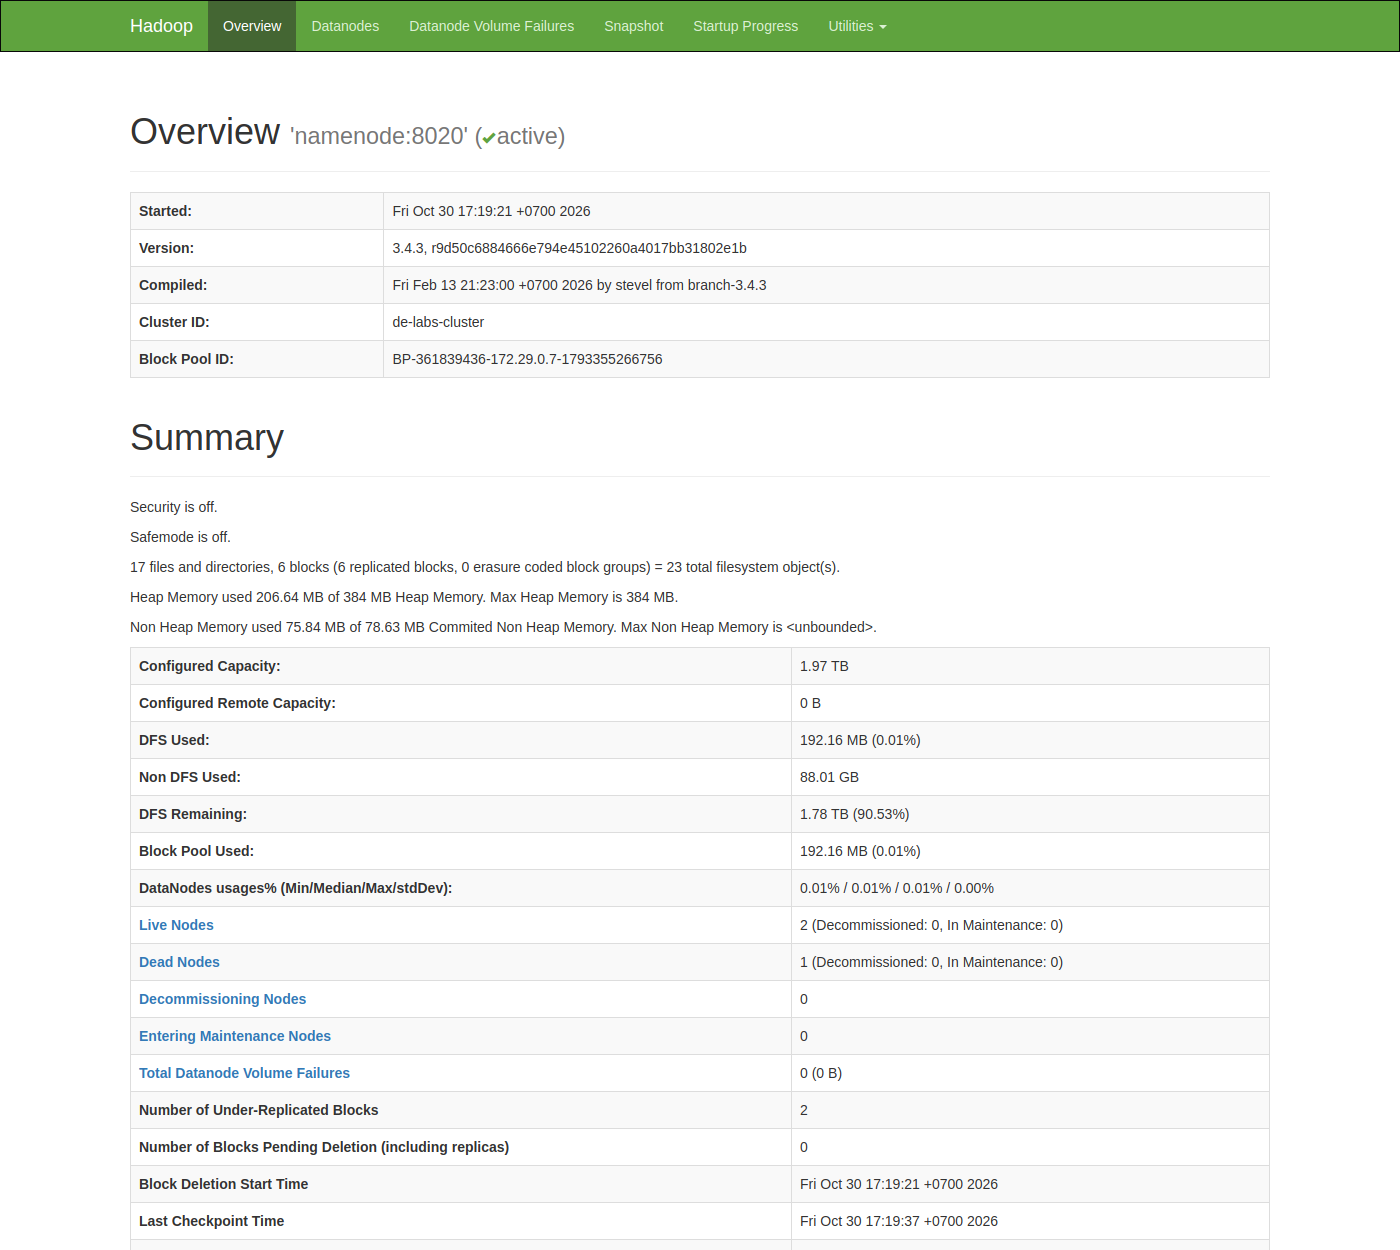
\includegraphics[width=1\linewidth,height=\textheight,keepaspectratio]{img/14_ui_overview_datanode3_DEAD.png}
\caption{Trang Overview của NameNode khi datanode3 đã bị tuyên bố
chết.}\label{fig:l01-ui-dead-overview}
\end{figure}

\begin{figure}
\centering
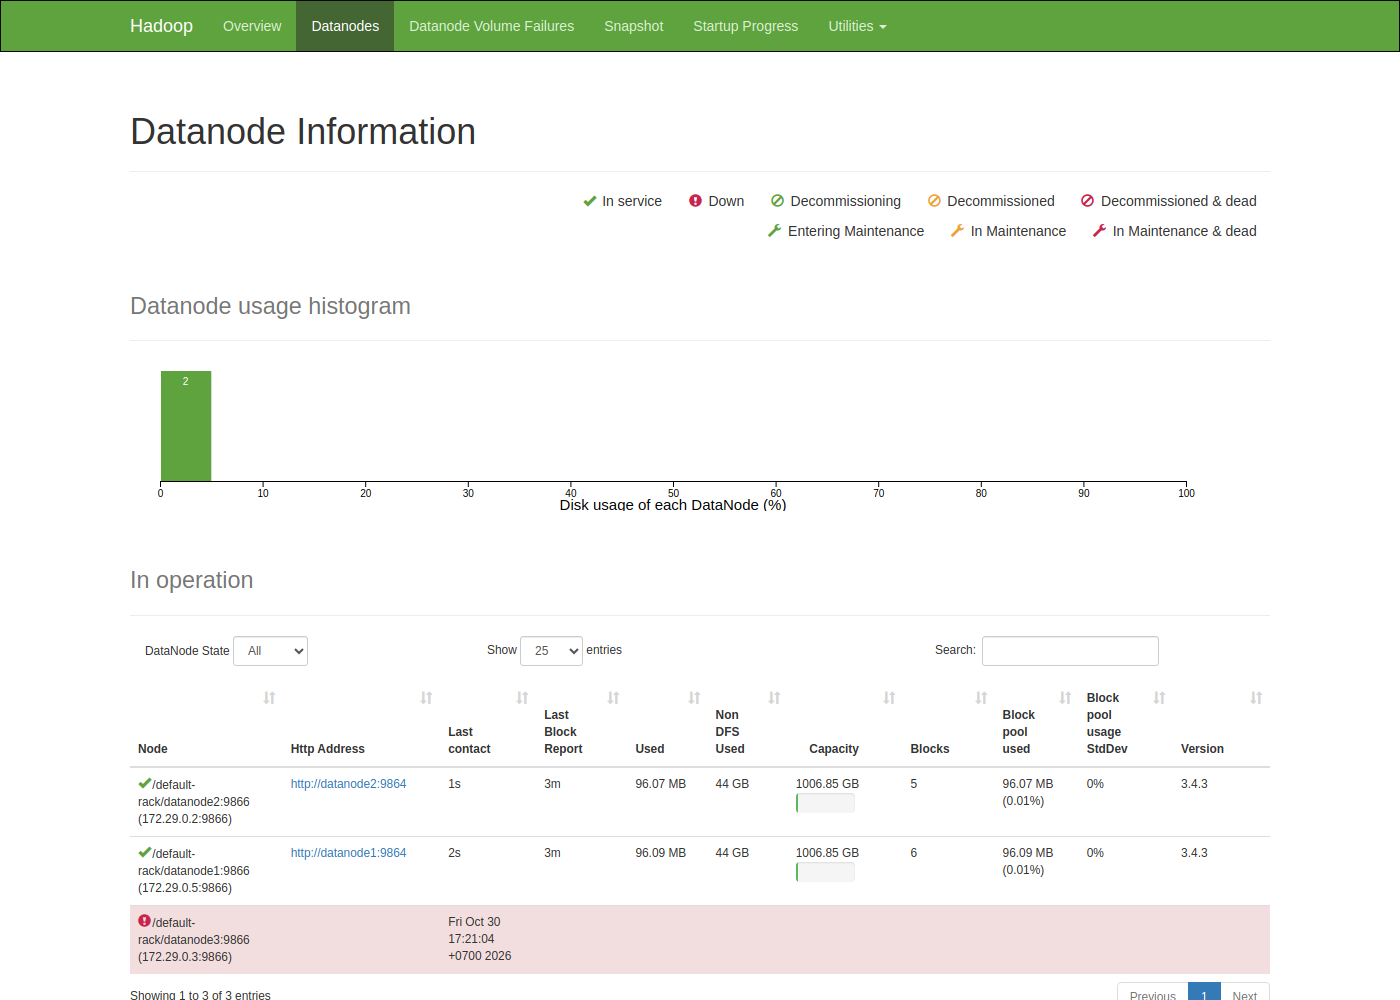
\includegraphics[width=1\linewidth,height=\textheight,keepaspectratio]{img/15_ui_datanodes_datanode3_DEAD.png}
\caption{Trang Datanodes khi datanode3 chết: datanode1 và datanode2 In
service, datanode3 ở trạng thái Down.}\label{fig:l01-ui-dead-datanodes}
\end{figure}

\texttt{fsck} lúc 10:18:38 cho thấy \texttt{small\_blocks} đã trở lại
\texttt{OK}:
\texttt{Number\ of\ data-nodes:}\allowbreak{}\texttt{\ 2}\allowbreak{},
cả ba block \texttt{Live\_repl=2},
\texttt{Under-replicated\ blocks:}\allowbreak{}\texttt{\ 0}\allowbreak{}
(Hình~\ref{fig:l01-after}). Replica trên datanode3 đã được chép sang
datanode2, node còn sống duy nhất chưa giữ bản sao
(Bảng~\ref{tbl:l01-locations}).

\begin{longtable}[]{@{}
  >{\raggedright\arraybackslash}p{(\linewidth - 6\tabcolsep) * \real{0.2500}}
  >{\raggedright\arraybackslash}p{(\linewidth - 6\tabcolsep) * \real{0.2500}}
  >{\raggedright\arraybackslash}p{(\linewidth - 6\tabcolsep) * \real{0.2500}}
  >{\raggedright\arraybackslash}p{(\linewidth - 6\tabcolsep) * \real{0.2500}}@{}}
\caption{\label{tbl:l01-locations}Vị trí replica của tệp
\texttt{small\_blocks} (hệ số 2) trước và sau khi dừng
datanode3.}\tabularnewline
\toprule\noalign{}
\begin{minipage}[b]{\linewidth}\raggedright
Block
\end{minipage} & \begin{minipage}[b]{\linewidth}\raggedright
Kích thước (byte)
\end{minipage} & \begin{minipage}[b]{\linewidth}\raggedright
Trước sự cố
\end{minipage} & \begin{minipage}[b]{\linewidth}\raggedright
Sau sự cố
\end{minipage} \\
\midrule\noalign{}
\endfirsthead
\toprule\noalign{}
\begin{minipage}[b]{\linewidth}\raggedright
Block
\end{minipage} & \begin{minipage}[b]{\linewidth}\raggedright
Kích thước (byte)
\end{minipage} & \begin{minipage}[b]{\linewidth}\raggedright
Trước sự cố
\end{minipage} & \begin{minipage}[b]{\linewidth}\raggedright
Sau sự cố
\end{minipage} \\
\midrule\noalign{}
\endhead
\bottomrule\noalign{}
\endlastfoot
\texttt{blk\_1073741828} & 16,777,216 & datanode1, datanode3 &
datanode1, datanode2 \\
\texttt{blk\_1073741829} & 16,777,216 & datanode3, datanode1 &
datanode1, datanode2 \\
\texttt{blk\_1073741830} & 16,407,209 & datanode3, datanode1 &
datanode1, datanode2 \\
\end{longtable}

\begin{figure}
\centering
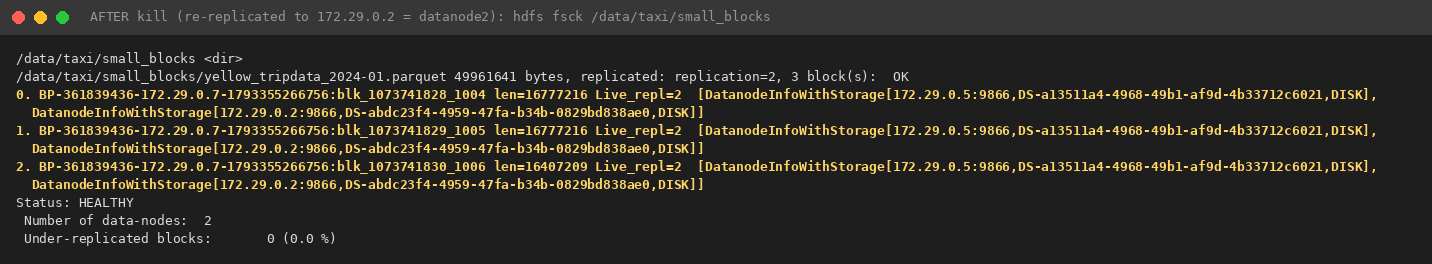
\includegraphics[width=0.85\linewidth,height=\textheight,keepaspectratio]{img/07_fsck_small_blocks_AFTER_kill.png}
\caption{\texttt{fsck} của tệp block 16 MB sau khi dừng datanode3:
replica đã chuyển sang datanode2, tệp trở lại trạng thái
OK.}\label{fig:l01-after}
\end{figure}

Với toàn bộ \texttt{/data}, \texttt{fsck} báo
\textbf{\texttt{Under-replicated\ blocks:}\allowbreak{}\texttt{\ 2\ (40.}\allowbreak{}\texttt{0\ \%)}\allowbreak{}}
(2 trên 5 block) và \texttt{Status:\ HEALTHY}
(Hình~\ref{fig:l01-underrep}). Hai block này thuộc hai tệp hệ số 3, mỗi
block còn 2 replica trên datanode2 và datanode1
(Bảng~\ref{tbl:l01-underrep}). Tệp Parquet hệ số 3 tải về có md5
\texttt{10dff36f5a2fc325274438bf361c70f0}\allowbreak{}, trùng với bản
gốc. Tệp
\texttt{/}\allowbreak{}\texttt{tmp/}\allowbreak{}\texttt{one\_}\allowbreak{}\texttt{replica.}\allowbreak{}\texttt{csv}\allowbreak{}
không bị MISSING vì replica duy nhất của nó nằm trên datanode1.

\begin{longtable}[]{@{}
  >{\raggedright\arraybackslash}p{(\linewidth - 8\tabcolsep) * \real{0.2000}}
  >{\raggedright\arraybackslash}p{(\linewidth - 8\tabcolsep) * \real{0.2000}}
  >{\raggedright\arraybackslash}p{(\linewidth - 8\tabcolsep) * \real{0.2000}}
  >{\raggedright\arraybackslash}p{(\linewidth - 8\tabcolsep) * \real{0.2000}}
  >{\raggedright\arraybackslash}p{(\linewidth - 8\tabcolsep) * \real{0.2000}}@{}}
\caption{\label{tbl:l01-underrep}Trạng thái các tệp trong \texttt{/data}
khi chỉ còn 2 DataNode sống.}\tabularnewline
\toprule\noalign{}
\begin{minipage}[b]{\linewidth}\raggedright
Tệp
\end{minipage} & \begin{minipage}[b]{\linewidth}\raggedright
Hệ số đích
\end{minipage} & \begin{minipage}[b]{\linewidth}\raggedright
Block
\end{minipage} & \begin{minipage}[b]{\linewidth}\raggedright
\texttt{Live\_repl}
\end{minipage} & \begin{minipage}[b]{\linewidth}\raggedright
Trạng thái
\end{minipage} \\
\midrule\noalign{}
\endfirsthead
\toprule\noalign{}
\begin{minipage}[b]{\linewidth}\raggedright
Tệp
\end{minipage} & \begin{minipage}[b]{\linewidth}\raggedright
Hệ số đích
\end{minipage} & \begin{minipage}[b]{\linewidth}\raggedright
Block
\end{minipage} & \begin{minipage}[b]{\linewidth}\raggedright
\texttt{Live\_repl}
\end{minipage} & \begin{minipage}[b]{\linewidth}\raggedright
Trạng thái
\end{minipage} \\
\midrule\noalign{}
\endhead
\bottomrule\noalign{}
\endlastfoot
\texttt{default\_}\allowbreak{}\texttt{blocks/}\allowbreak{}\texttt{.}\allowbreak{}\texttt{.}\allowbreak{}\texttt{.}\allowbreak{}\texttt{parquet}\allowbreak{}
& 3 & \texttt{blk\_1073741827} & 2 & Under replicated \\
\texttt{small\_}\allowbreak{}\texttt{blocks/}\allowbreak{}\texttt{.}\allowbreak{}\texttt{.}\allowbreak{}\texttt{.}\allowbreak{}\texttt{parquet}\allowbreak{}
& 2 & 3 block & 2 & OK \\
\texttt{taxi\_}\allowbreak{}\texttt{zone\_}\allowbreak{}\texttt{lookup.}\allowbreak{}\texttt{csv}\allowbreak{}
& 3 & \texttt{blk\_1073741825} & 2 & Under replicated \\
\end{longtable}

\begin{figure}
\centering
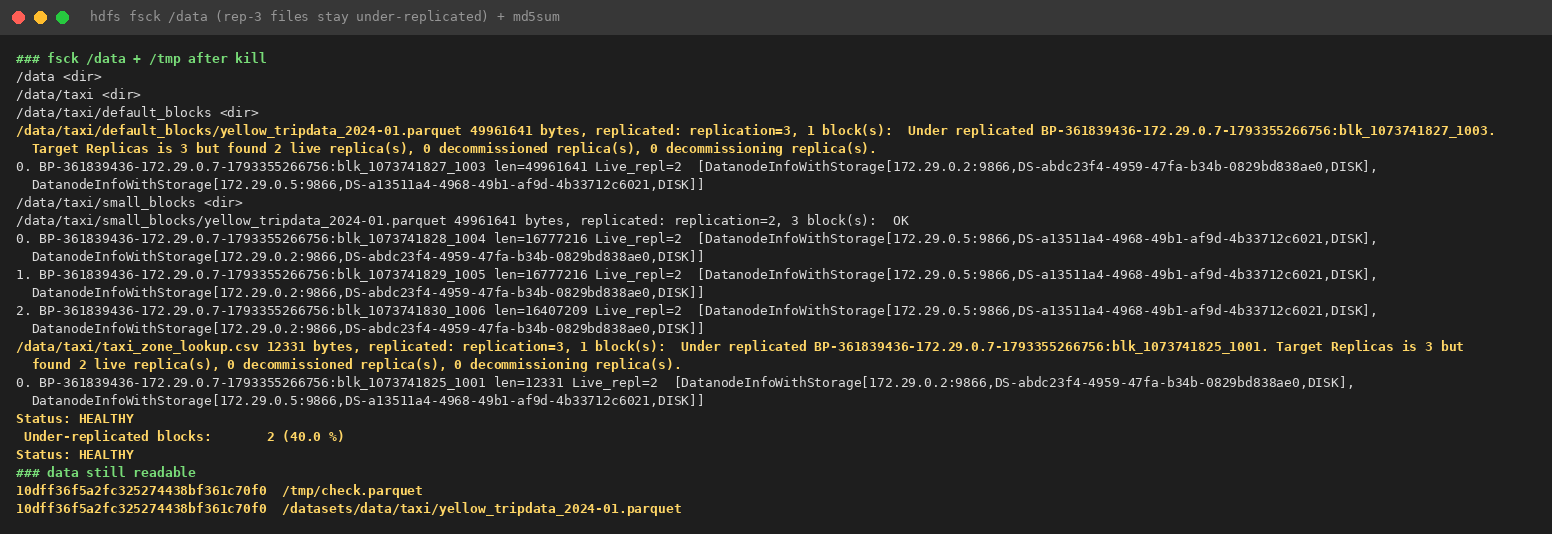
\includegraphics[width=0.85\linewidth,height=\textheight,keepaspectratio]{img/08_fsck_data_underreplicated_md5.png}
\caption{\texttt{fsck\ /data} khi datanode3 chết: hai tệp hệ số 3
under-replicated nhưng HEALTHY; md5 của tệp tải về trùng bản
gốc.}\label{fig:l01-underrep}
\end{figure}

Khởi động lại datanode3, \texttt{dfsadmin\ -report}\allowbreak{} trở về
\texttt{Live\ datanodes\ (3)}\allowbreak{} và \texttt{fsck} báo
\texttt{Under-replicated\ blocks:}\allowbreak{}\texttt{\ 0}\allowbreak{},
\texttt{Over-replicated\ blocks:}\allowbreak{}\texttt{\ 0}\allowbreak{},
\texttt{Status:\ HEALTHY} (Hình~\ref{fig:l01-back}). Các block hệ số 3
đã có lại replica thứ ba; tệp hệ số 2 lúc này có replica trên cả ba
node, và NameNode đã xóa bớt bản thừa.

\begin{figure}
\centering
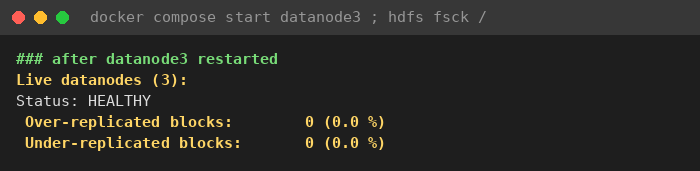
\includegraphics[width=0.7\linewidth,height=\textheight,keepaspectratio]{img/09_datanode3_back.png}
\caption{Trạng thái cluster sau khi datanode3 quay lại: không còn block
under-replicated hay over-replicated.}\label{fig:l01-back}
\end{figure}

\subsection{Safe mode và fsimage}\label{sec:l01-safemode}

Khi bật safe mode thủ công, lệnh ghi bị từ chối với thông báo
\texttt{put:}\allowbreak{}\texttt{\ Cannot\ create\ file/}\allowbreak{}\texttt{tmp/}\allowbreak{}\texttt{x.}\allowbreak{}\texttt{csv.}\allowbreak{}\texttt{\_}\allowbreak{}\texttt{COPYING\_}\allowbreak{}\texttt{.}\allowbreak{}\texttt{\ Name\ node\ is\ in\ safe\ mode.}\allowbreak{},
còn
\texttt{hdfs\ dfs\ -ls\ /}\allowbreak{}\texttt{data/}\allowbreak{}\texttt{taxi}\allowbreak{}
vẫn trả về 3 mục (Hình~\ref{fig:l01-safemode}). Sau
\texttt{docker\ compose\ restart\ namenode}\allowbreak{},
\texttt{-safemode\ get} báo \texttt{Safe\ mode\ is\ ON} trong vài giây
đầu rồi chuyển sang OFF khi tỉ lệ block được báo cáo đạt ngưỡng 99.9 \%
(\texttt{threshold-pct}) cộng 5 s extension.

\texttt{saveNamespace} tạo
\texttt{fsimage\_}\allowbreak{}\texttt{0000000000000000059}\allowbreak{}
dung lượng 1,574 byte (kèm \texttt{.md5} 62 byte, \texttt{seen\_txid} 3
byte, \texttt{VERSION} 189 byte). Bản XML do \texttt{hdfs\ oiv} sinh ra
có tên thư mục và tệp (\texttt{tmp}, \texttt{hadoop-yarn},
\texttt{user}, \texttt{root}, \texttt{data}, \texttt{taxi},
\texttt{taxi\_}\allowbreak{}\texttt{zone\_}\allowbreak{}\texttt{lookup.}\allowbreak{}\texttt{csv}\allowbreak{},
\ldots) cùng block ID, nhưng tìm thông tin DataNode (cổng 9866) thì được
0 dòng: fsimage không chứa vị trí block.

\begin{figure}
\centering
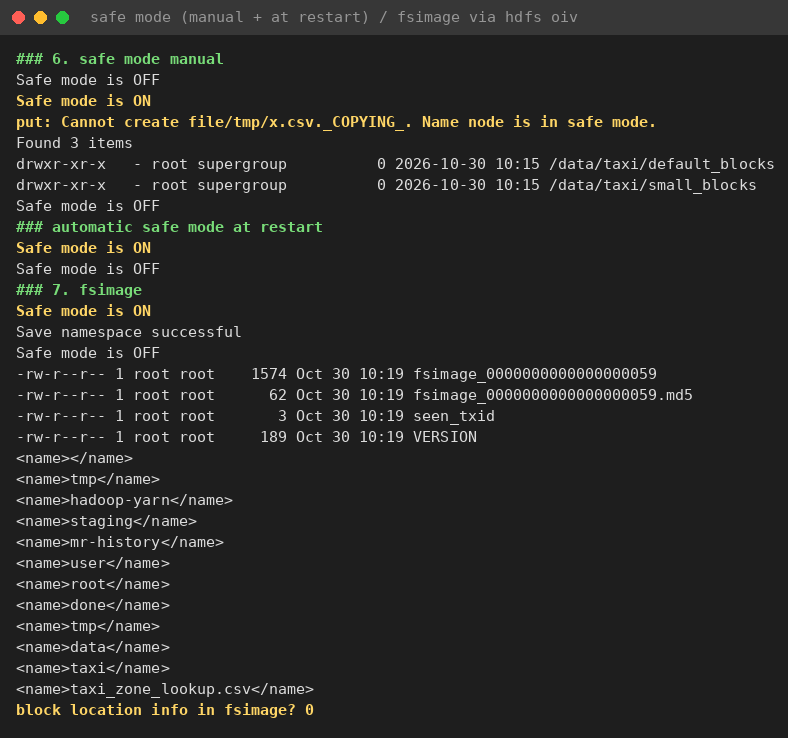
\includegraphics[width=0.85\linewidth,height=\textheight,keepaspectratio]{img/10_safemode_fsimage.png}
\caption{Safe mode thủ công (ghi bị từ chối, đọc vẫn hoạt động), safe
mode tự động khi khởi động lại và nội dung
fsimage.}\label{fig:l01-safemode}
\end{figure}

\section{Trả lời câu hỏi checkpoint}\label{sec:l01-discussion}

\subsection{Tệp 300 MB với cấu hình mặc định chiếm bao nhiêu block,
replica và dung lượng?}\label{sec:l01-q1}

Số block là \(\lceil 300/128 \rceil = 3\): hai block 128 MB và một block
cuối 44 MB. Với hệ số 3 có \(3 \times 3 = 9\) replica và khoảng
\(3 \times 300 = 900\) MB dung lượng thô, cộng thêm tệp \texttt{.meta}
khoảng 0.78 \% (Bảng~\ref{tbl:l01-physical}). Block cuối không chiếm
trọn 128 MB (Mục~\ref{sec:l01-q2}), và phép nhân ba dung lượng khớp với
số đo ở Bảng~\ref{tbl:l01-du}.

\subsection{Vì sao block cuối của tệp taxi nhỏ hơn 16 MB, và có tốn 16
MB đĩa không?}\label{sec:l01-q2}

Vì tệp kết thúc ở đó:
\(49{,}961{,}641 - 2 \times 16{,}777{,}216 = 16{,}407{,}209\) byte. Tệp
\texttt{blk\_1073741830} trên datanode1 đúng bằng kích thước này
(Bảng~\ref{tbl:l01-physical}), nên không có phần đĩa nào bị bỏ phí, khác
với block của hệ thống tệp cục bộ (ví dụ 4 KB) vốn được cấp phát trọn.
Tệp 12,331 byte được gán block size 128 MB cũng chỉ chiếm 12,331 byte
trên mỗi DataNode.

\subsection{Vị trí block được lưu ở đâu, và khi NameNode khởi động lại
thì sao?}\label{sec:l01-q3}

Ánh xạ block sang DataNode chỉ nằm trong RAM của NameNode: fsimage có
tên tệp và block ID nhưng không có thông tin DataNode nào
(Mục~\ref{sec:l01-safemode}, Hình~\ref{fig:l01-safemode}). Khi khởi động
lại, NameNode nạp namespace từ fsimage và edit log rồi dựng lại block
map từ block report, nên phải ở safe mode cho tới khi nhận đủ báo cáo.
Thiết kế này hợp lý vì chỉ DataNode mới biết chắc block nào đang nằm
trên đĩa của nó; trong lúc NameNode tắt, đĩa có thể hỏng hoặc node bị
thay, nên danh sách vị trí lưu sẵn sẽ nhanh chóng sai {[}1{]}, {[}2{]}.
Hiện tượng thiếu replica tạm thời ngay sau khi ghi
(Mục~\ref{sec:l01-blocksize}) cũng xuất phát từ đây.

\subsection{Vì sao tệp hệ số 2 được phục hồi còn tệp hệ số 3 thì
không?}\label{sec:l01-q4}

Muốn tái nhân bản phải có một DataNode còn sống chưa giữ replica của
block, vì HDFS không đặt hai replica của cùng block trên một node
{[}3{]}. Mỗi block của tệp hệ số 2 ban đầu nằm trên datanode1 và
datanode3, nên datanode2 còn trống để nhận bản sao mới
(Bảng~\ref{tbl:l01-locations}, Hình~\ref{fig:l01-after}). Block của hai
tệp hệ số 3 thì đã có mặt trên cả hai node còn sống
(Bảng~\ref{tbl:l01-underrep}), không còn chỗ cho bản thứ ba, nên phải
chờ datanode3 quay lại (Hình~\ref{fig:l01-back}). Số replica tối đa đạt
được là \(\min(\text{hệ số đích}, \text{số DataNode sống})\).

\subsection{\texorpdfstring{\texttt{fsck} báo gì khi có block
under-replicated, và vì sao đó chưa phải
lỗi?}{fsck báo gì khi có block under-replicated, và vì sao đó chưa phải lỗi?}}\label{sec:l01-q5}

\texttt{fsck\ /data} vẫn báo \texttt{Status:\ HEALTHY} khi có block
under-replicated (Hình~\ref{fig:l01-underrep}). HEALTHY nghĩa là mọi
block còn ít nhất
\texttt{dfs.}\allowbreak{}\texttt{namenode.}\allowbreak{}\texttt{replication.}\allowbreak{}\texttt{min}\allowbreak{}
(= 1) replica sống, nên dữ liệu vẫn đọc được, và md5 trùng khớp ở
Mục~\ref{sec:l01-failure} xác nhận điều này. Under-replication chỉ làm
giảm độ dư thừa: hỏng thêm một node thì các block này còn một bản. Lỗi
thật là MISSING hoặc CORRUPT, khi block không còn replica hợp lệ nào;
\texttt{/}\allowbreak{}\texttt{tmp/}\allowbreak{}\texttt{one\_}\allowbreak{}\texttt{replica.}\allowbreak{}\texttt{csv}\allowbreak{}
sẽ rơi vào trường hợp này nếu replica duy nhất của nó nằm trên
datanode3.

\subsection{\texorpdfstring{Nếu giữ
\texttt{recheck-interval}\allowbreak{} mặc định 5 phút thì sao, và vì
sao timeout dài lại
tốt?}{Nếu giữ recheck-interval mặc định 5 phút thì sao, và vì sao timeout dài lại tốt?}}\label{sec:l01-q6}

Theo công thức ở Mục~\ref{sec:l01-failure}, node sẽ bị tuyên bố chết sau
\(2 \times 300 + 10 \times 3 = 630\) s, tức 10.5 phút, thay vì 90 s như
Bảng~\ref{tbl:l01-timeline}. Trong môi trường thật, timeout dài tránh
được \emph{replication storm} (bão tái nhân bản): một node khởi động lại
để vá lỗi hoặc mất mạng một phút cũng có thể kéo theo việc sao chép hàng
terabyte block, và khi node quay lại thì các bản sao đó thành thừa,
trong khi băng thông và I/O đĩa bị tiêu tốn đúng lúc cluster đang không
ổn định. Hai ngưỡng phục vụ hai việc khác nhau: ngưỡng stale ngắn (mặc
định 30 s, trong lab 15 s) giúp client tránh node bất thường gần như
ngay, còn ngưỡng dead dài chỉ quyết định lúc bắt đầu tái nhân bản, việc
tốn kém nhất.

\subsection{Vì sao NameNode khởi động trong safe mode và phải chặn
ghi?}\label{sec:l01-q7}

Lúc khởi động, NameNode biết namespace nhưng chưa biết block nằm ở đâu
(Mục~\ref{sec:l01-q3}), nên khi chưa đủ 99.9 \% block được báo cáo, nó
không phân biệt được block thật sự mất với block chỉ chưa kịp báo. Nếu
cho ghi, xóa hay tái nhân bản lúc này, NameNode có thể sao chép hàng
loạt block chưa được báo cáo hoặc xóa nhầm replica tưởng là thừa. Safe
mode giữ hệ thống chỉ đọc cho tới khi block map đáng tin
(Mục~\ref{sec:l01-safemode}).

\subsection{Vì sao 1 triệu tệp 1 KB là vấn đề, còn 1 tệp 1 KB thì
không?}\label{sec:l01-q8}

Mỗi tệp, thư mục và block là một đối tượng trong heap NameNode, khoảng
150 byte mỗi đối tượng {[}4{]}. Một triệu tệp nhỏ tạo ít nhất 2 triệu
đối tượng (một inode và một block mỗi tệp), xấp xỉ 300 MB heap cho
khoảng 1 GB dữ liệu. Khi ghi còn có 1 triệu lời gọi RPC tới NameNode, và
khi xử lý bằng MapReduce thì có 1 triệu map task vì mỗi tệp tạo ít nhất
một split (\emph{small files problem}). Trong thực nghiệm, tệp 12,331
byte vẫn chiếm riêng một block ID và một replica trên mỗi DataNode
(Bảng~\ref{tbl:l01-physical}). Cách xử lý thường dùng là gộp tệp nhỏ
thành tệp lớn hoặc dùng định dạng chứa như Parquet/ORC, SequenceFile,
HAR.

\section{Kết luận}\label{sec:l01-conclusion}

Bài lab đã hoàn thành các bước 1 đến 7 của đề. Block size chỉ là giới
hạn trên và dung lượng thô tỉ lệ với hệ số nhân bản. Khi dừng datanode3,
node bị tuyên bố chết sau 90 s như công thức, tệp hệ số 2 tự tái nhân
bản sang datanode2, còn hai tệp hệ số 3 under-replicated nhưng vẫn
HEALTHY và đọc được. fsimage không chứa vị trí block, đó là lý do
NameNode cần safe mode khi khởi động.

\section*{Tài liệu tham khảo}\label{tuxe0i-liux1ec7u-tham-khux1ea3o}
\addcontentsline{toc}{section}{Tài liệu tham khảo}

{[}1{]} S. Ghemawat, H. Gobioff, and S.-T. Leung, ``The Google File
System,'' in \emph{Proc. 19th ACM Symposium on Operating Systems
Principles (SOSP)}, 2003, pp.~29-43.

{[}2{]} K. Shvachko, H. Kuang, S. Radia, and R. Chansler, ``The Hadoop
Distributed File System,'' in \emph{Proc. IEEE 26th Symposium on Mass
Storage Systems and Technologies (MSST)}, 2010, pp.~1-10.

{[}3{]} Apache Software Foundation, ``HDFS Architecture,'' Apache Hadoop
3.4 Documentation.
https://hadoop.apache.org/docs/stable/hadoop-project-dist/hadoop-hdfs/HdfsDesign.html

{[}4{]} T. White, \emph{Hadoop: The Definitive Guide}, 4th
ed.~Sebastopol, CA, USA: O'Reilly Media, 2015.

{[}5{]} Apache Software Foundation, ``hdfs-default.xml,'' Apache Hadoop
3.4 Documentation.
https://hadoop.apache.org/docs/stable/hadoop-project-dist/hadoop-hdfs/hdfs-default.xml

\section*{Phụ lục: Tệp nộp kèm và trích đoạn
lệnh}\label{phux1ee5-lux1ee5c-tux1ec7p-nux1ed9p-kuxe8m-vuxe0-truxedch-ux111oux1ea1n-lux1ec7nh}
\addcontentsline{toc}{section}{Phụ lục: Tệp nộp kèm và trích đoạn lệnh}

Các log nộp kèm được liệt kê ở Bảng~\ref{tbl:l01-files}; ảnh chụp nằm
trong \texttt{img/}.

\begin{longtable}[]{@{}
  >{\raggedright\arraybackslash}p{(\linewidth - 2\tabcolsep) * \real{0.5000}}
  >{\raggedright\arraybackslash}p{(\linewidth - 2\tabcolsep) * \real{0.5000}}@{}}
\caption{\label{tbl:l01-files}Danh mục tệp log nộp kèm báo
cáo.}\tabularnewline
\toprule\noalign{}
\begin{minipage}[b]{\linewidth}\raggedright
Tệp
\end{minipage} & \begin{minipage}[b]{\linewidth}\raggedright
Nội dung
\end{minipage} \\
\midrule\noalign{}
\endfirsthead
\toprule\noalign{}
\begin{minipage}[b]{\linewidth}\raggedright
Tệp
\end{minipage} & \begin{minipage}[b]{\linewidth}\raggedright
Nội dung
\end{minipage} \\
\midrule\noalign{}
\endhead
\bottomrule\noalign{}
\endlastfoot
\texttt{01\_}\allowbreak{}\texttt{shell\_}\allowbreak{}\texttt{blocks.}\allowbreak{}\texttt{txt}\allowbreak{}
& \texttt{dfsadmin\ -report}\allowbreak{}, lệnh \texttt{hdfs\ dfs},
\texttt{-stat}, \texttt{fsck} block 128 MB/16 MB, tệp block \\
\texttt{02\_setrep.txt} & \texttt{fsck} tệp 16 MB khi đã ổn định,
\texttt{setrep\ -w\ 2}, \texttt{du\ -h}, ghi tệp hệ số 1 \\
\texttt{03\_} đến \texttt{07\_*.txt} & \texttt{fsck} trước/sau khi dừng
datanode3, dòng thời gian, md5, datanode3 quay lại \\
\texttt{08\_}\allowbreak{}\texttt{safemode\_}\allowbreak{}\texttt{fsimage.}\allowbreak{}\texttt{txt}\allowbreak{}
& Safe mode thủ công và tự động, \texttt{saveNamespace}, phân tích
fsimage \\
\end{longtable}

In tên, block size, hệ số nhân bản và kích thước của
\texttt{taxi\_}\allowbreak{}\texttt{zone\_}\allowbreak{}\texttt{lookup.}\allowbreak{}\texttt{csv}\allowbreak{}:

\begin{Shaded}
\begin{Highlighting}[]
\ExtensionTok{hdfs}\NormalTok{ dfs }\AttributeTok{{-}stat} \StringTok{"name=\%n blocksize=\%o repl=\%r size=\%b"}\NormalTok{ /data/taxi/taxi\_zone\_lookup.csv}
\CommentTok{\# name=taxi\_zone\_lookup.csv blocksize=134217728 repl=3 size=12331}
\end{Highlighting}
\end{Shaded}

Ghi tệp với hệ số 1 trong một lệnh, không dùng \texttt{setrep}:

\begin{Shaded}
\begin{Highlighting}[]
\ExtensionTok{hdfs}\NormalTok{ dfs }\AttributeTok{{-}D}\NormalTok{ dfs.replication=1 }\AttributeTok{{-}put}\NormalTok{ /datasets/data/taxi/taxi\_zone\_lookup.csv /tmp/one\_replica.csv}
\CommentTok{\# one\_replica.csv repl=1   (replica duy nhất trên 172.29.0.5 = datanode1)}
\end{Highlighting}
\end{Shaded}

Các lệnh chính của thí nghiệm block và sự cố DataNode:

\begin{Shaded}
\begin{Highlighting}[]
\ExtensionTok{hdfs}\NormalTok{ dfs }\AttributeTok{{-}D}\NormalTok{ dfs.blocksize=16m }\AttributeTok{{-}put}\NormalTok{ /datasets/data/taxi/yellow\_tripdata\_2024{-}01.parquet }\DataTypeTok{\textbackslash{}}
\NormalTok{    /data/taxi/small\_blocks/}
\ExtensionTok{hdfs}\NormalTok{ fsck /data/taxi/small\_blocks }\AttributeTok{{-}files} \AttributeTok{{-}blocks} \AttributeTok{{-}locations}
\ExtensionTok{hdfs}\NormalTok{ dfs }\AttributeTok{{-}setrep} \AttributeTok{{-}w}\NormalTok{ 2 /data/taxi/small\_blocks/yellow\_tripdata\_2024{-}01.parquet}
\ExtensionTok{docker}\NormalTok{ compose stop datanode3          }\CommentTok{\# chạy trên máy host}
\ControlFlowTok{while} \FunctionTok{true}\KeywordTok{;} \ControlFlowTok{do} \ExtensionTok{hdfs}\NormalTok{ dfsadmin }\AttributeTok{{-}report} \KeywordTok{|} \FunctionTok{grep} \AttributeTok{{-}E} \StringTok{"Live|Dead|Under"}\KeywordTok{;} \FunctionTok{sleep}\NormalTok{ 5}\KeywordTok{;} \ControlFlowTok{done}
\ExtensionTok{hdfs}\NormalTok{ dfs }\AttributeTok{{-}get}\NormalTok{ /data/taxi/default\_blocks/yellow\_tripdata\_2024{-}01.parquet /tmp/check.parquet}
\FunctionTok{md5sum}\NormalTok{ /tmp/check.parquet /datasets/data/taxi/yellow\_tripdata\_2024{-}01.parquet}
\end{Highlighting}
\end{Shaded}


\end{document}
